\documentclass[compress]{beamer}
\usepackage[utf8x]{inputenc}
\usepackage{default}
\usepackage{graphics}
\usepackage{ulem}
\usepackage{multicol}

\useinnertheme{rounded}
\usecolortheme{whale}
\useoutertheme[subsection=false]{miniframes}
\setbeamertemplate{footline}[frame number]
\beamertemplatenavigationsymbolsempty

%%%%%%%% begin tikz %%%%%%
\usepackage{tikz}
\usetikzlibrary{shapes.callouts,decorations.pathmorphing}
\usetikzlibrary{shapes,decorations,shadows}
\usetikzlibrary{decorations.pathmorphing}
\usetikzlibrary{decorations.shapes}
\usetikzlibrary{fadings}
\usetikzlibrary{patterns}
\usetikzlibrary{calc}
\usetikzlibrary{decorations.text}
\usetikzlibrary{decorations.footprints}
\usetikzlibrary{decorations.fractals}
\usetikzlibrary{shapes.gates.logic.IEC}
\usetikzlibrary{shapes.gates.logic.US}
\usetikzlibrary{fit,chains}
\usetikzlibrary{positioning}
\usepgflibrary{shapes}
\usetikzlibrary{scopes}
\usetikzlibrary{arrows}
\usetikzlibrary{backgrounds}


\pgfdeclarelayer{background}
\pgfdeclarelayer{foreground}
\pgfsetlayers{background,main,foreground}

\tikzset{latent/.style={circle,fill=white,draw=red,thick,inner sep=1pt, 
minimum size=20pt, font=\fontsize{10}{10}\selectfont},
obs/.style={latent,fill=gray!25},
const/.style={rectangle, inner sep=0pt},
factor/.style={rectangle, fill=red,minimum size=7pt, inner sep=0pt},
yellow/.style={latent,minimum size=15pt,fill=yellow!75},
blue/.style={latent,minimum size=15pt,fill=blue!75},
-/.style={color=red, thick},
>={triangle 45}}




% shapename, fitlist, caption, pos
\newcommand{\plate}[4]{
\node (invis#1) [draw, transparent, inner sep=1pt,rectangle,fit=#2] {};
\node (capt#1) [ below left=0 pt of invis#1.south east, xshift=0pt,yshift=-9pt] {\raisebox{0pt}[0pt]{\footnotesize{#3}}};
\node (#1) [draw=black!50,thick,inner sep=3pt,rectangle,rounded corners,fit=(invis#1) (capt#1),#4] {};
}


\newcommand{\shiftedplate}[5]{
\node (invis#1) [draw, transparent, inner sep=0 pt,rectangle,fit=#2] {};
\node (capt#1) [#5, xshift=2pt] {\footnotesize{#3}};
\node (#1) [draw,inner sep=2pt, rectangle,fit=(invis#1) (capt#1),#4] {};
}
%shapename, pos, caption, in, out, captpos
\newcommand{\factor}[6]{
\node (#1) [factor] at #2 {};
\node (capt#1) [#6 of #1]{\footnotesize{#3}};
\draw [-] (#4) -- (#1) ;
\draw [->,thick] (#1) -- (#5);
}

% name, --, caption, pos
\newcommand{\nofactor}[4]{
\node (#1) [factor, #2]  {};
\node (capt#1) [#4 of #1]{\footnotesize{#3}};
}


\title{Novelty Detection for Semantic Place Categorization}
\author{André Susano Pinto\inst{1,2}}
\date{18 July 2011}

\institute {
 Supervised by: Andrzej Pronobis\inst{1}, Luis Paulo Reis\inst{2}
 \and
 \inst{1}The Royal Institute of Technology (KTH), Sweden \\
 \inst{2}Faculdade de Engenharia da Universidade do Porto
}

\begin{document}
\begin{frame}
 \titlepage
\end{frame}

\begin{frame}{Outline}
  \begin{multicols}{2}
    \tableofcontents
  \end{multicols}
\end{frame}



\section{Introduction}
\subsection{Motivation}
\begin{frame}{Motivation}

\begin{columns}[t]
  \column{0.3\textwidth}
  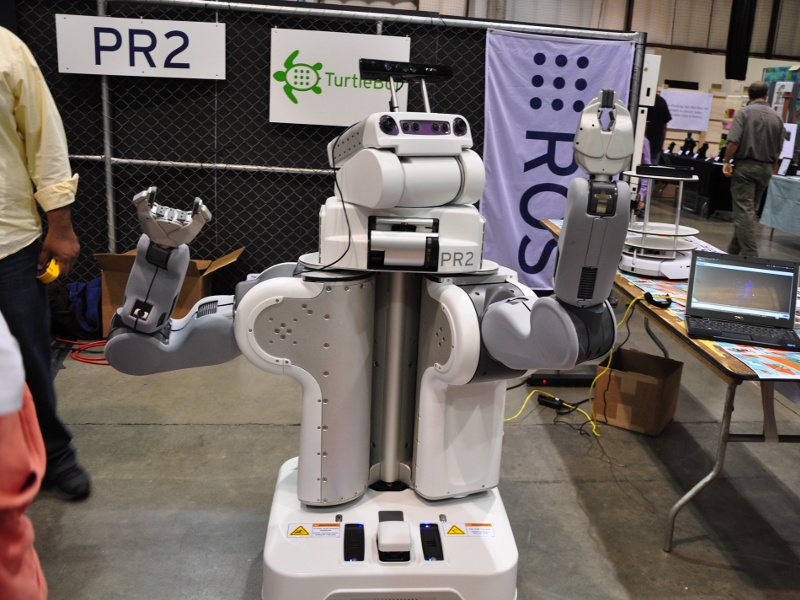
\includegraphics[width=\textwidth]{figures/extra/PR2.jpg}

  \centering
  PR2

  \column{0.3\textwidth}
  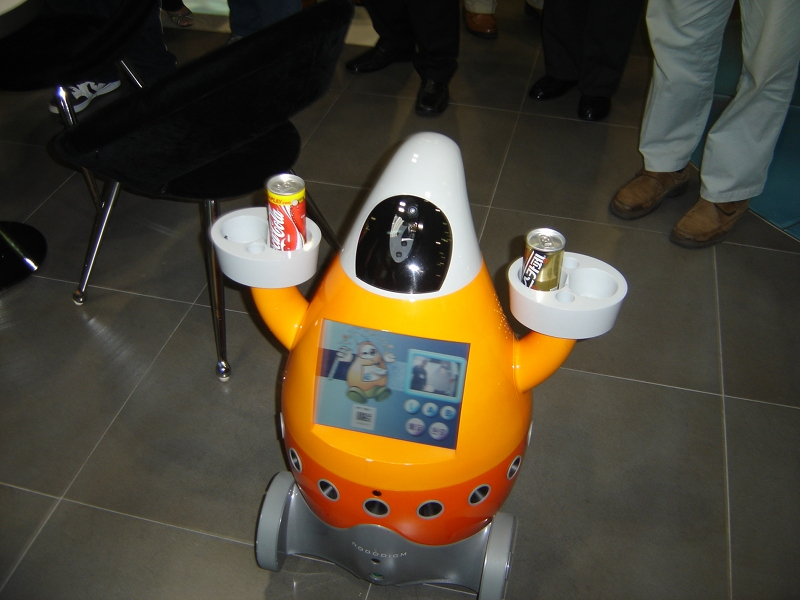
\includegraphics[width=\textwidth]{figures/extra/servingbot.jpg}
  
  \centering
  Serving Robot

  \column{0.3\textwidth}
  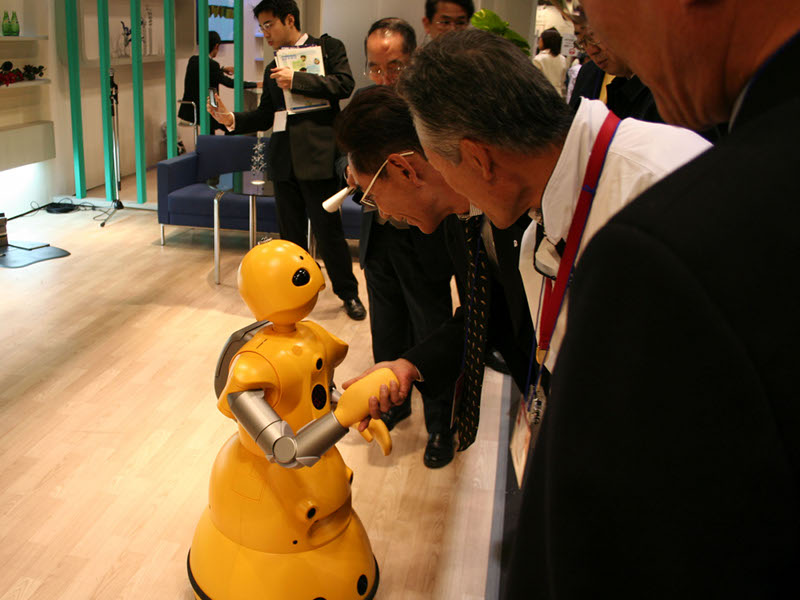
\includegraphics[width=\textwidth]{figures/extra/wakamaru.jpg}
  
  \centering
  Wakamaru
\end{columns}
\vfill

\begin{itemize}
  \item Robots are useful: can make our lives easier
  \item Robots are entering our Houses and Offices
  \item They need to understand our world and communicate with us.
\end{itemize}
\note{
1 - Humans dream on creating robots. 
Both by the challenge on creating intelligent systems on itself but also to make our life easier.
% I should have an example list on how they could be useful

2 - It is becoming a reality and robots will enter our houses and offices.
The question is no longer if we will have a robot at home/office, but how many.

3 - They will need to understand and communicate with us and our human worlds.
The need of semantic information!
}
\end{frame}


\subsection{Problem}
\begin{frame}{Problem}

  Enhance world with semantic information is \alert{not a scalable solution}.

  \begin{block}{}
  \begin{columns}
  \column{0.3\textwidth}
    \begin{figure}
      \includegraphics[width=\textwidth]{figures/extra/RFID.pdf} \\
      RFID for object tagging
    \end{figure}
  \column{0.3\textwidth}
    \begin{figure}
      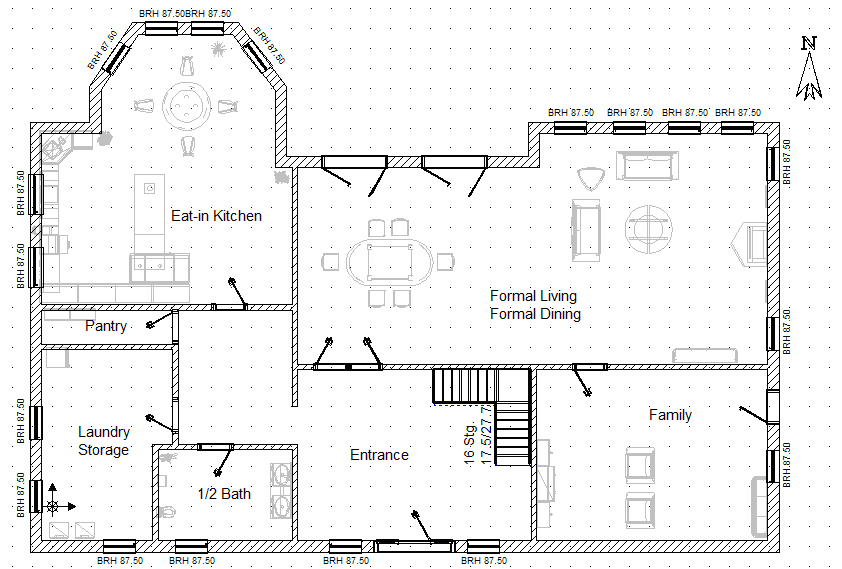
\includegraphics[width=\textwidth]{figures/extra/floorplan.jpg} \\
      Maps extended with semantic information
    \end{figure}
  \end{columns}
  \end{block}

\note{
1 - A solution could pass by tagging our world with extra information, such as maps, rfids, but such a solution
is not practical and scalable.
}
\end{frame}

\begin{frame}{Problem}
\begin{block}{Machine Learning}
Give us methods to solve this problem in reverse by providing robots with knowledge
on how to detect and classify concepts and categories from the underlying sensed world.
\end{block}

\begin{block}{Unreliable on Dynamic and Unknown Environments}
It is unrealistic to believe on the possibility to fully describe the required knowledge
for the agent in all situations.
\end{block}

\note{
Machine Learning tries to solve the reverse semantic mapping problem.

It endows robots with knowledge that allows them to map what they sense to human concepts
and categories.

Leading to the need of methods that are able to inspect and smartly identifying information directly
from low-level sensors.

For that several machine learning techniques have been developed, but all of those require and represent
knowledge that is given a-priori.
}
\end{frame}

\begin{frame}{Problem}

\begin{block}{Detection of Knowledge-Gaps}
Detection of situations where the agent knowledge does not suffices.
\end{block}

\begin{block}{Focus on Semantic Categories of Places}
Humans attribute meaning to the areas that describe the expected properties,
objects and actions of them. E.g.\ cups are found in kitchens. 
\end{block}
\note{
- It is unrealistic to believe on the possibility to describe all the required knowledge

- When dealing with novel and unknown scenarios an agent has to be able to detect something
is not conforming to what it has learn.

In order to be reliable agents need to detect situations where their knowledge
And agents be reliable even when situations
- Scalability
- Dynamic Aspects
- Long Term
- Life Long


It is unrealistic to believe on the possibility to describe knowledge that holds to all the possible
scenarios, and when dealing with long-term and life-long agents

- Variability, dynamic aspects of environment, 
- Should be able to deal with novel cases
- 1st step is to detect them
}
\end{frame}

\subsection{Goals}
\begin{frame}{Goals}
  \begin{itemize}
    \item Study a semantic mapping process in the context of mobile robots \cite{pronobis2011phd}.
    \item Propose a method based on the studied system to detect novel semantic categories of places.
  \end{itemize}

\note{
This thesis goes on the direction of detecting knowledge gaps on mobile robots.

It studies a process of semantic mapping introduced by Pronobis
and studies how to detect those situations where the existent knowledge does not describes
the reality.
But being such a large problem, this thesis focus then specifically on detecting novel room categories.
}
\end{frame}

\subsection{Outline}
\begin{frame}{Outline}
  \begin{multicols}{2}
    \tableofcontents
  \end{multicols}
\end{frame}


%%%%%%%%%%%%%%%%%%%%%%%%%%%%%%%%%%%%%%%%%%%%%%%%%%%%%%%%%%%%%%%%%%%%%%%%%%%%
\section{Semantic Mapping}

\subsection{Mapping}
\begin{frame}{Mapping - Machine Friendly}
\begin{columns}[tc]
\column{0.5\textwidth}
  \begin{figure}
    \only<1>{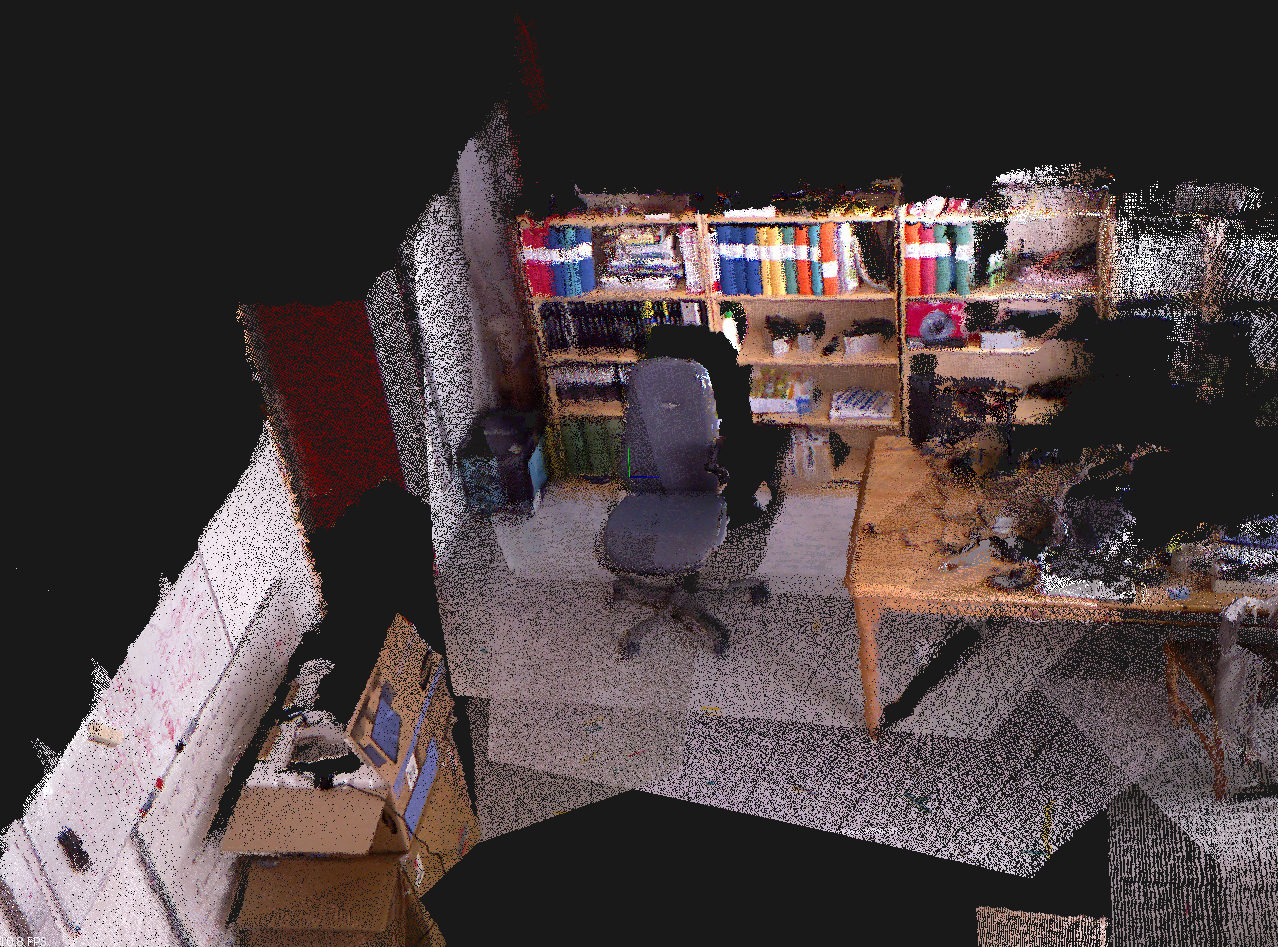
\includegraphics[width=\textwidth]{figures/extra/pointcloud.jpg}}
    \only<2>{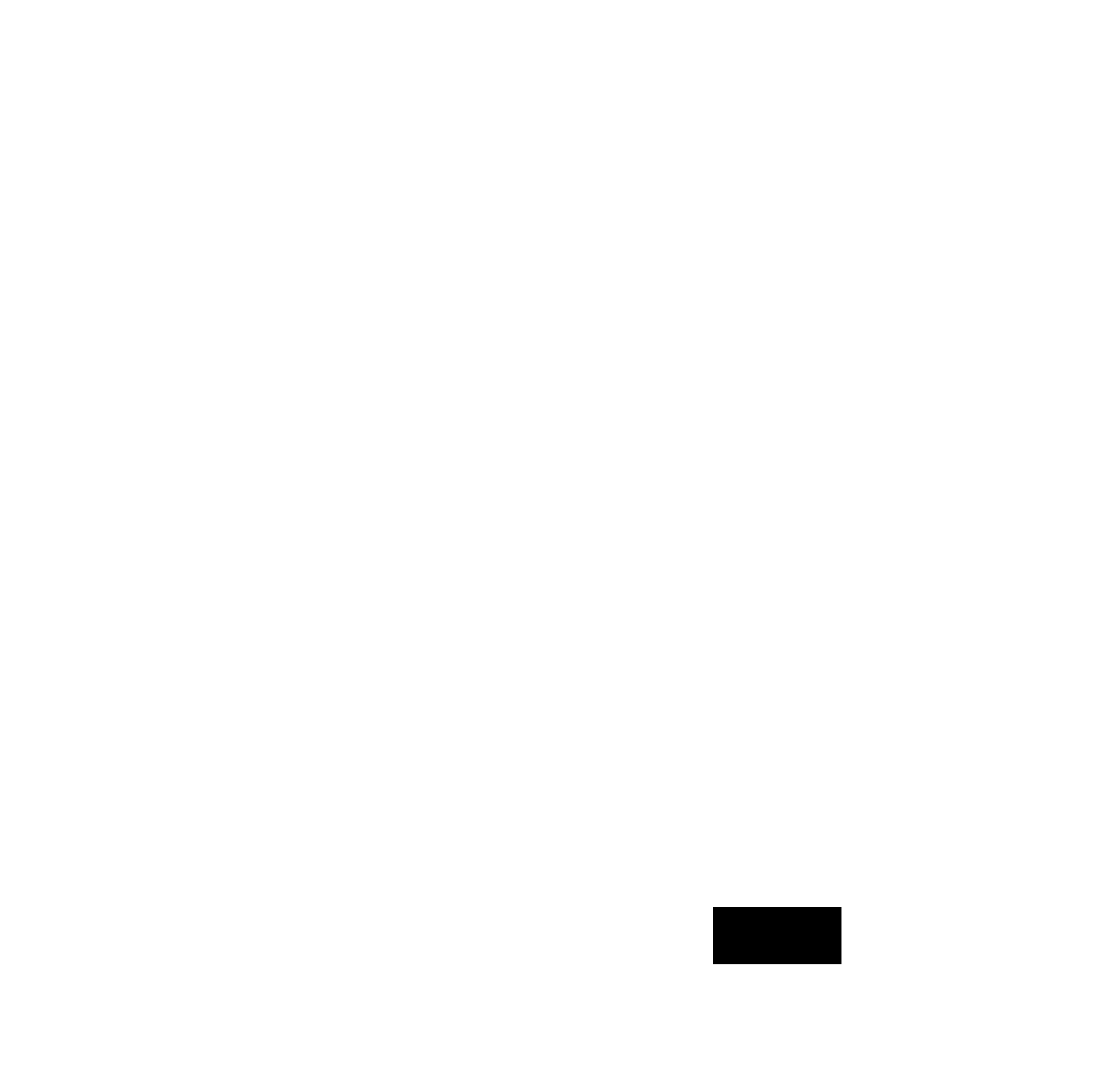
\includegraphics[width=\textwidth]{figures/machinefriendly.pdf}}
  \end{figure}

\column{0.5\textwidth}
  \only<1>{
  \begin{itemize}
    \item World Representation
    \item Bypass Sensory Horizon
    \item Planning Tool
  \end{itemize}
  }

  \only<2>{
  \begin{tikzpicture}
    % \draw [help lines] grid(3,2);

    \node (human) at (0,0) {\reflectbox{
\includegraphics[width=0.4\textwidth]{figures/extra/bart.pdf}}};
    \node (robot) at (3,0) {\reflectbox{\includegraphics[width=0.2\textwidth]{figures/robot.png}}};

    \node[ellipse callout, draw, callout absolute pointer={(human.70)}]
          (humanvoice) at (1,3) {Where is Wally?};

    \node[ellipse callout, draw, callout absolute pointer={(robot.north)},
          text width=0.2\textwidth]
          (robotvoice) at (3,2) {X=32, Y=17};

  \end{tikzpicture}
  }
\end{columns}
\end{frame}

\subsection{Semantic Mapping}
\begin{frame}{Semantic Mapping}
\begin{columns}[tt]

\column{0.5\textwidth}
  \begin{figure}
    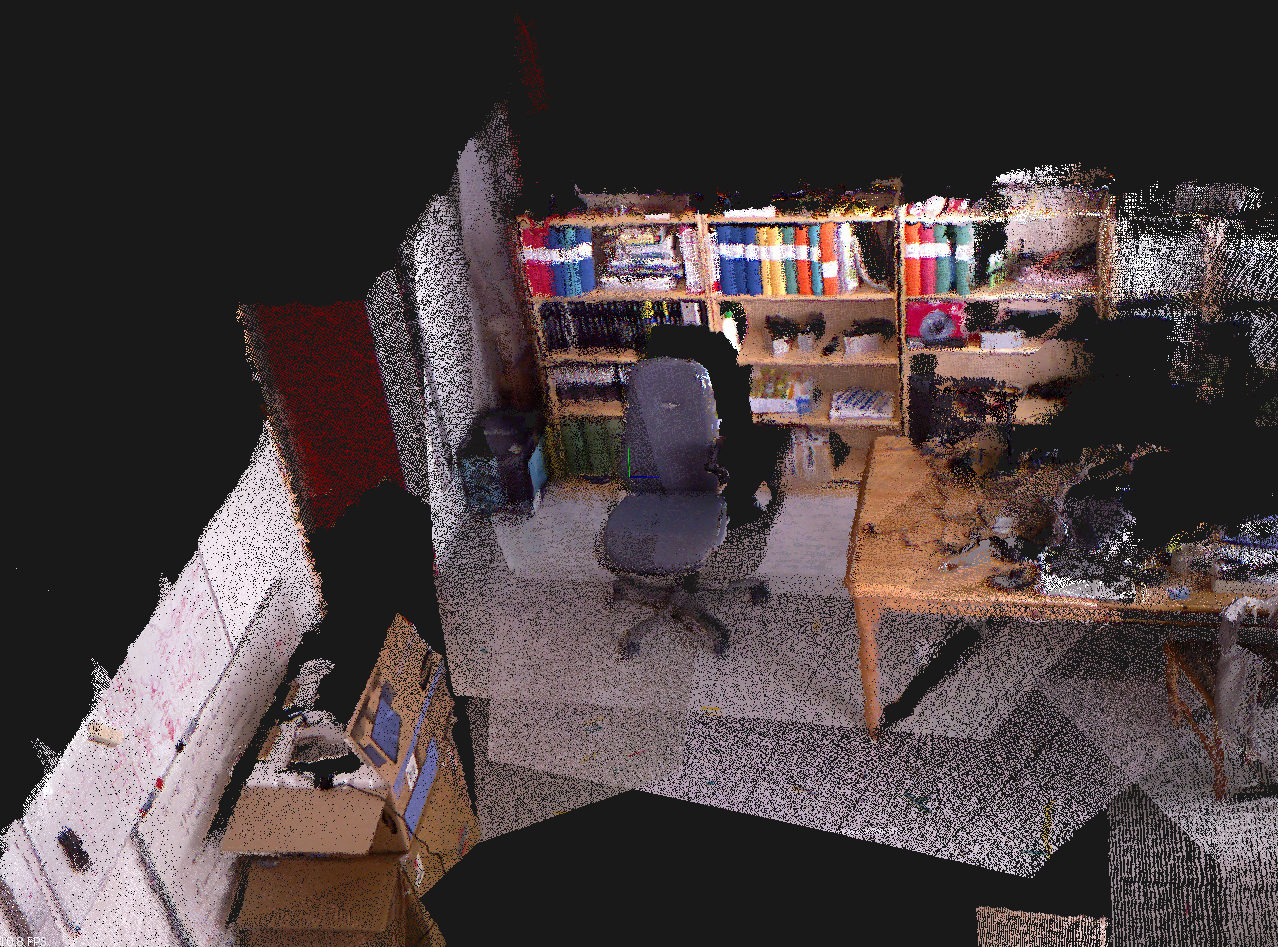
\includegraphics[width=\textwidth]{figures/semanticfriendly.pdf}
  \end{figure}

\column{0.5\textwidth}
  \only<1>{
  \begin{figure}
  \begin{tikzpicture}
    \node (human) at (0,0) {\reflectbox{
\includegraphics[width=0.4\textwidth]{figures/extra/bart.pdf}}};
    \node (robot) at (3,0) {\reflectbox{\includegraphics[width=0.2\textwidth]{figures/robot.png}}};

    \node[ellipse callout, draw, callout absolute pointer={(human.70)}]
          (humanvoice) at (1,3) {Where is Wally?};

    \node[ellipse callout, draw, callout absolute pointer={(robot.north)},
          text width=0.2\textwidth]
          (robotvoice) at (3,2) {In the office};

  \end{tikzpicture}
  \end{figure}
  }

  \only<2>{
  \begin{itemize}
    \item High Level Reasoning
    \item Easier Planning \cite{hanheide2011ijcai}
    \item Closer to Human Semantic
  \end{itemize}
  }

\end{columns}
\end{frame}

\subsection{Spatial Knowledge}
\begin{frame}{Spatial Knowledge}
  \begin{columns}[c]
  \column{0.5\textwidth}
    \begin{figure}
    \includegraphics[width=0.8\textwidth]{figures/spatial-knowledge-representation.pdf}
    \end{figure}

  \column{0.5\textwidth}
    \begin{block}{Layered Spatial Knowledge Representation~\cite{pronobis2010ias}}
    \begin{itemize}
      \item Sensory Layer
      \item Place Layer
      \item Categorical Layer
      \item Conceptual Layer
    \end{itemize}
    \end{block}
  \end{columns}
\end{frame}

\subsection{Process}
\begin{frame}{A Semantic Mapping Process}
  \begin{figure}
    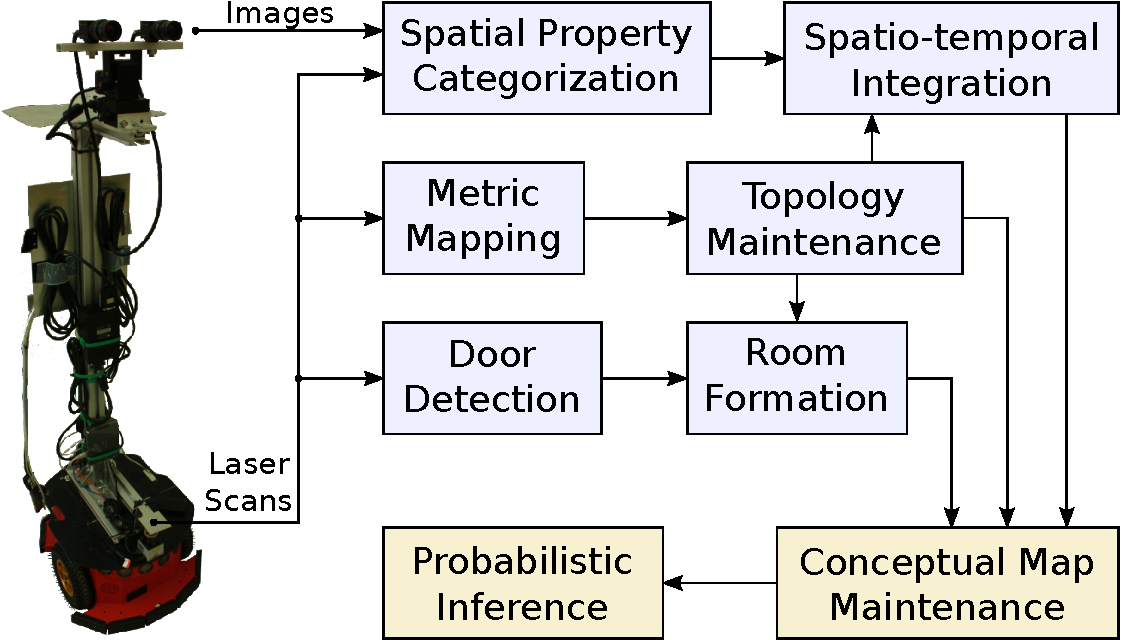
\includegraphics[width=0.8\textwidth]{figures/dora-architecture.pdf}
  \end{figure}
  \cite{pronobis2011semmap} presents a process that uses the spatial knowledge
  to perform probabilistic and multi-modal semantic mapping of the environment
  using graphical models.
\end{frame}

\subsection{Conceptual Map}
\begin{frame}{Conceptual Map}
  \begin{columns}[c]
  \column{0.5\textwidth}
    \begin{figure}
      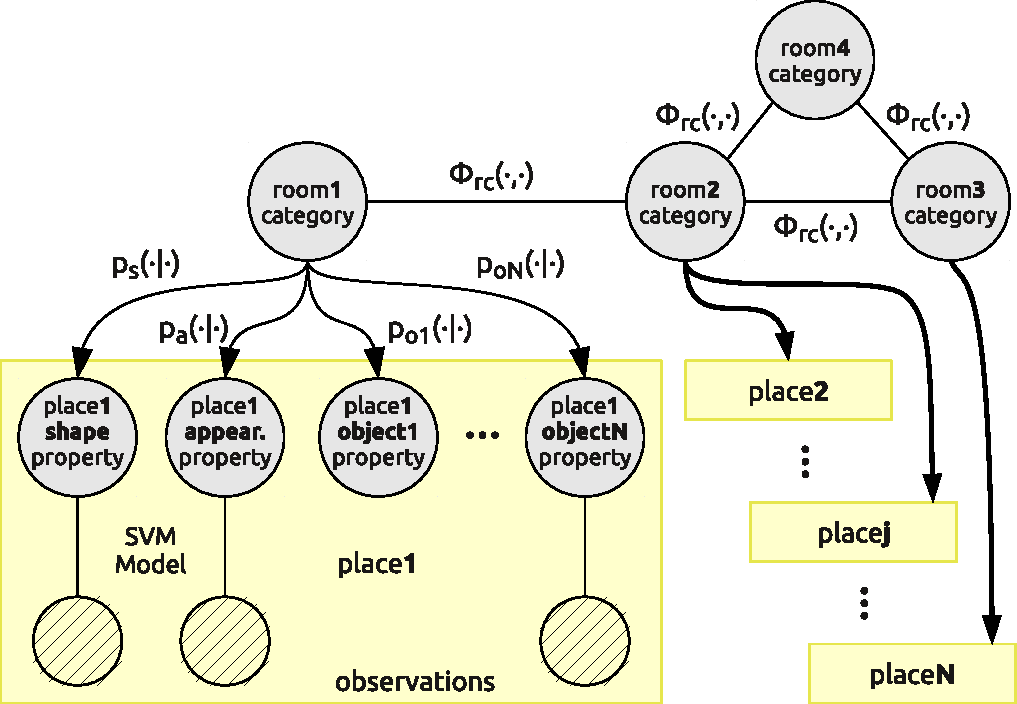
\includegraphics[width=\textwidth]{figures/chaingraph.pdf}
    \end{figure}
  \column{0.5\textwidth}
    \begin{itemize}
      \item Uncertain Ontology
      \item Probabilistic Inference
      \item Use of Graphical Models
    \end{itemize}
  \end{columns}

  \note{
    The semantic mapping process proposed by Pronobis uses the previously presented spatial knowledge
    to produce a conceptual map that relates all the identified concepts and relates them ...


    This tool allows to perform semantic mapping of the environment, but is not able to handle gaps
    on the agent knowledge.
  }
\end{frame}

\begin{frame}{Probabilistic Graphical Models}
Provides us methods to relate and combine the several information,
Can be approximated, handle uncertainties, etc\dots

\begin{block}{Several Methods}
Bayes Networks, Random Markov Fields, Chain Graphs, Factor Graphs
\end{block}

\end{frame}


%%%%%%%%%%%%%%%%%%%%%%%%%%%%%%%%%%%%%%%%%%%%%%%%%%%%%%%%%%%%%%%%%%%%%%%%%%%%%%%%%%%
\section{Novelty Detection}

\subsection{Fast Review}
\begin{frame}{Novelty Detection - Fast Review}
  \begin{block}{Definition}
    Detection of novel patterns or signals presents on the data that the system was not trained
    to handle -- \cite{markou2003novelty}
  \end{block}
  \begin{block}{Single Class Classification}
    Lack of negative samples makes them suitable for cases where it is not possible to
    provide negative samples: anomaly detection, intrusion detection, etc\dots
  \end{block}
  \begin{block}{Several Methods}
    K-PCA, One class SVM, Nearest Neighbours, etc\dots
  \end{block}
\end{frame}

\subsection{Thresholding}
\begin{frame}{Novelty Detection via Thresholding}

\begin{block}{Threshold on Probability Density}
For a fixed distribution and without any prior knowledge on the distribution,
novelty can be detected by thresholding on the density of
the training data as shown on \cite{bishop1994novelty}.
\end{block}

\begin{block}{Dynamic Sample Space}
As more information becomes available the probability mass spreads around and
the threshold for novelty detection needs to be adjusted.
\alert<2->{How to do it?}
\end{block}
\end{frame}

\subsection{Conditional and Unconditional Ratio}
\begin{frame}{Ordering the Sample Space}
\begin{block}{Back to the Roots}
An optimal detector can be implemented by defining a threshold over a
relation order defined by $P(\overline{novel}|x)$.
\end{block}
\vfill

\begin{block}{Conditional and Unconditional Probability Ratio}
\[P(\overline{novel}|x) = \frac{P(x|\overline{novel})P(\overline{novel})}{P(x)} \propto \frac{P(x|\overline{novel})}{P(x)}\]
\uncover<2>{\alert{Simplified with an assumption on constant $P(novel)$}}
\end{block}
\note{
Going back to a definition of a novelty detector, it can be shown that any optimal
detector can be seen as a solving a continuous knapsack problem, and that a threshold
can be set over the order relation defined by the probability of a sample being novel.
}
\end{frame}

\subsection{Models}
\begin{frame}{Conditional Probability}
\begin{columns}[c]
  \column{0.5\textwidth}
    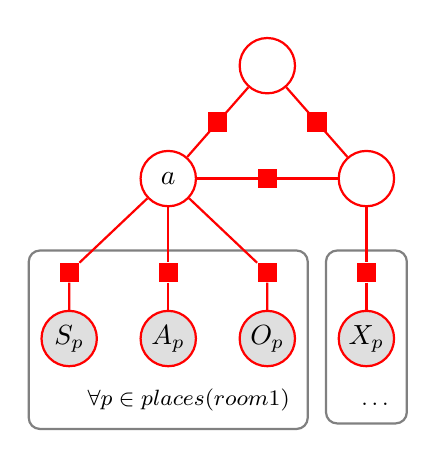
\begin{tikzpicture}
  \node [matrix,matrix anchor=mid, column sep=15pt, row sep=10pt,ampersand replacement=\&] {
    \& \& \node (room3) [latent] {}; \& \\
    \& \& \& \\
    \&
    \node (room1) [latent] {$a$}; \& \&
    \node (room2) [latent] {}; \\
    \& \& \& \\
    \node (shape1f) [factor] {}; \&
    \node (appearance1f) [factor] {}; \&
    \node (object1f) [factor] {}; \&
    \node (factor2) [factor] {}; \\
    \node (shape1l) [obs] {$S_p$}; \&
    \node (appearance1l) [obs] {$A_p$}; \&
    \node (object1l) [obs] {$O_p$}; \&
    \node (prop2) [obs] {$X_p$}; \\
  };

  \draw [-] (room1) -- (shape1f) -- (shape1l);
  \draw [-] (room1) -- (appearance1f) -- (appearance1l);
  \draw [-] (room1) -- (object1f) -- (object1l);
  \draw [-] (room2) -- (factor2) -- (prop2);

  \draw [-] (room1) -- (room2) node (r12f) [midway,factor] {};
  \draw [-] (room1) -- (room3) node (r13f) [midway,factor] {};
  \draw [-] (room2) -- (room3) node (r23f) [midway,factor] {};

  \begin{pgfonlayer}{background}
    \plate{places1}{(shape1f)(shape1l)(object1l)}{$\forall p \in places(room1)$}{};
    \plate{places2}{(factor2)(prop2)}{$\dots$}{};
  \end{pgfonlayer}
\end{tikzpicture}

  \column{0.5\textwidth}
    \begin{block}{$P(x|\overline{novel})$}
      The graphical model used by the conceptual map represents the distribution of the
      variables given that the agent knowledge holds true.

%      The conditional probability is then the probability of the sensed features being
%      generated by a distribution modelled according to the agent knowledge.
    \end{block}
\end{columns}
\end{frame}

\begin{frame}{Unconditional Probability Model}
\only<1>{
\begin{columns}[t]
  \column{0.5\textwidth}
  \begin{tikzpicture}
  \node [matrix,matrix anchor=mid, column sep=15pt, row sep=10pt,ampersand replacement=\&] {
    \& \& \node (room3) [latent] {}; \& \\
    \& \& \& \\
    \&
    \node (room1) [latent] {}; \& \&
    \node (room2) [latent] {}; \\
    \& \& \& \\
    \&
    \&
    \&
    \\
    \node (shape1l) [obs] {$S_p$}; \&
    \node (appearance1l) [obs] {$A_p$}; \&
    \node (object1l) [obs] {$O_p$}; \&
    \node (prop2) [obs] {$X_p$}; \\
  };

  \begin{pgfonlayer}{background}
    \plate{places1}{(shape1f)(shape1l)(object1l)}{$\forall p \in places(room1)$}{};
    \plate{places2}{(factor2)(prop2)}{$\dots$}{};
  \end{pgfonlayer}
\end{tikzpicture}

  
  \centering
  No prior knowledge on $P(x)$. \\
  Uniform distribution~\cite{shore1980axiomatic}

\column{0.5\textwidth}
  \begin{tikzpicture}
  \node [matrix,matrix anchor=mid, column sep=15pt, row sep=10pt,ampersand replacement=\&] {
    \& \& \node (room3) [latent] {}; \& \\
    \& \& \& \\
    \&
    \node (room1) [factor] {}; \& \&
    \node (room2) [latent] {}; \\
    \& \& \& \\
    \&
    \&
    \&
    \node (factor2) [factor] {}; \\
    \node (shape1l) [obs] {$S_p$}; \&
    \node (appearance1l) [obs] {$A_p$}; \&
    \node (object1l) [obs] {$O_p$}; \&
    \node (prop2) [obs] {$X_p$}; \\
  };

  \draw [-] (room1) -- (shape1l);
  \draw [-] (room1) -- (appearance1l);
  \draw [-] (room1) -- (object1l);
  \draw [-] (room2) -- (prop2);

  \draw [-] (room1) -- (room2);
  \draw [-] (room1) -- (room3);
  \draw [-] (room2) -- (room3) node (r23f) [midway,factor] {};

  \begin{pgfonlayer}{background}
    \plate{places1}{(shape1f)(shape1l)(object1l)}{$\forall p \in places(room1)$}{};
    \plate{places2}{(factor2)(prop2)}{$\dots$}{};
  \end{pgfonlayer}
\end{tikzpicture}



  \centering
  Assume structure and knowledge on other variables still hold true on $P(x)$
\end{columns}
}
\only<2>{
\begin{columns}[c]
 \column{0.5\textwidth}
  \begin{tikzpicture}
  \node [matrix,matrix anchor=mid, column sep=15pt, row sep=10pt,ampersand replacement=\&] {
    \& \& \node (room3) [latent] {}; \& \\
    \& \& \& \\
    \&
    \node (room1) [factor] {}; \& \&
    \node (room2) [latent] {}; \\
    \& \& \& \\
    \&
    \&
    \&
    \node (factor2) [factor] {}; \\
    \node (shape1l) [obs] {$S_p$}; \&
    \node (appearance1l) [obs] {$A_p$}; \&
    \node (object1l) [obs] {$O_p$}; \&
    \node (prop2) [obs] {$X_p$}; \\
  };

  \draw [-,dashed] (room1) -- (shape1l);
  \draw [-,dashed] (room1) -- (appearance1l);
  \draw [-,dashed] (room1) -- (object1l);
  \draw [-] (room2) -- (prop2);

  \draw [-,dashed] (room1) -- (room2);
  \draw [-,dashed] (room1) -- (room3);
  \draw [-] (room2) -- (room3) node (r23f) [midway,factor] {};
  \node (captroom1) [above=0pt of room1] {\footnotesize{U}};

  \begin{pgfonlayer}{background}
    \plate{places1}{(shape1f)(shape1l)(object1l)}{$\forall p \in places(room1)$}{};
    \plate{places2}{(factor2)(prop2)}{$\dots$}{};
  \end{pgfonlayer}
\end{tikzpicture}



  \centering
  Uniform Model
 \column{0.5\textwidth}
  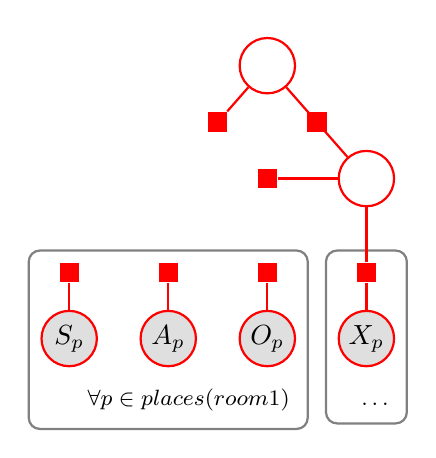
\begin{tikzpicture}
  \node [matrix,matrix anchor=mid, column sep=15pt, row sep=10pt,ampersand replacement=\&] {
    \& \& \node (room3) [latent] {}; \& \\
    \& \& \& \\
    \&
    \node (room1) [latent,draw=none] {}; \& \&
    \node (room2) [latent] {}; \\
    \& \& \& \\
    \node (shape1f) [factor] {}; \&
    \node (appearance1f) [factor] {}; \&
    \node (object1f) [factor] {}; \&
    \node (factor2) [factor] {}; \\
    \node (shape1l) [obs] {$S_p$}; \&
    \node (appearance1l) [obs] {$A_p$}; \&
    \node (object1l) [obs] {$O_p$}; \&
    \node (prop2) [obs] {$X_p$}; \\
  };

  \draw [-] (shape1f) -- (shape1l);
  \draw [-] (appearance1f) -- (appearance1l);
  \draw [-] (object1f) -- (object1l);
  \draw [-] (room2) -- (factor2) -- (prop2);

  \draw [-,draw=none] (room1) -- (room2) node (r12f) [midway,factor] {};
  \draw [-,draw=none] (room1) -- (room3) node (r13f) [midway,factor] {};
  \draw [-] (room2) -- (room3) node (r23f) [midway,factor] {};
  \draw [-] (room2) -- (r12f);
  \draw [-] (room3) -- (r13f);

  \begin{pgfonlayer}{background}
    \plate{places1}{(shape1f)(shape1l)(object1l)}{$\forall p \in places(room1)$}{};
    \plate{places2}{(factor2)(prop2)}{$\dots$}{};
  \end{pgfonlayer}
\end{tikzpicture}


  
  \centering
  Independent Model
\end{columns}
}
\end{frame}


\subsection{Results}
\begin{frame}{Synthetic Dataset}

\begin{columns}[c]
\column{0.5\textwidth}
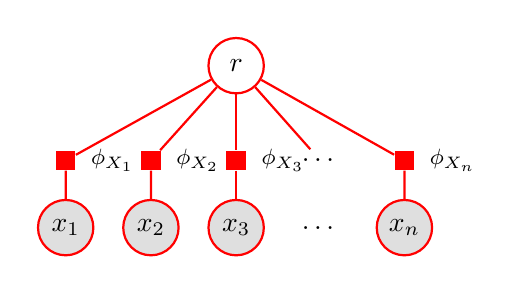
\begin{tikzpicture}
  \node [matrix,matrix anchor=mid, column sep=10pt, row sep=10pt,ampersand replacement=\&] {
    \& \& \node (room) [latent] {$r$}; \& \& \\
    \& \& \& \& \\
    \node (f1) [factor] {}; \&
    \node (f2) [factor] {}; \&
    \node (f3) [factor] {}; \&
    \node (fi) [] {\dots}; \&
    \node (fn) [factor] {}; \\
    \node (x1) [obs] {$x_1$}; \&
    \node (x2) [obs] {$x_2$}; \&
    \node (x3) [obs] {$x_3$}; \&
    \node (xi) [] {\dots}; \&
    \node (xn) [obs] {$x_n$}; \\
  };
  \draw [-] (room) -- (f1) -- (x1);
  \draw [-] (room) -- (f2) -- (x2);
  \draw [-] (room) -- (f3) -- (x3);
  \draw [-] (room) -- (fi);
  \draw [-] (room) -- (fn) -- (xn);

  \node (captf1) [right=2pt of f1] {\footnotesize{$\phi_{X_1}$}};
  \node (captf2) [right=2pt of f2] {\footnotesize{$\phi_{X_2}$}};
  \node (captf3) [right=2pt of f3] {\footnotesize{$\phi_{X_3}$}};
  \node (captfn) [right=2pt of fn] {\footnotesize{$\phi_{X_n}$}};
\end{tikzpicture}
\column{0.5\textwidth}

\begin{block}{Room class generator of features}
\begin{itemize}
  \item 11 - Room Categories
  \item 2 - Room Shapes (laser)
  \item 3 - Room Size (laser)
  \item 10 - Room Appearance (CRFH)
  \item 7 - Object Detectors (SIFT)
\end{itemize}
\end{block}
\end{columns}
\end{frame}


\begin{frame}{Synthetic Dataset - Conditional Model}
\begin{block}{Conditional Model}
\centering
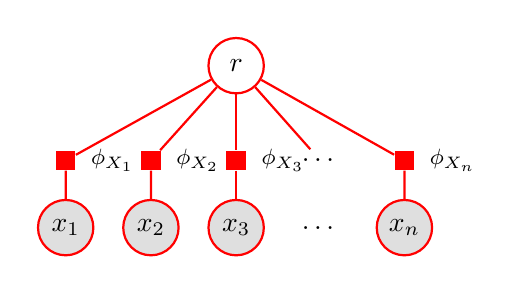
\begin{tikzpicture}
  \node [matrix,matrix anchor=mid, column sep=10pt, row sep=10pt,ampersand replacement=\&] {
    \& \& \node (room) [latent] {$r$}; \& \& \\
    \& \& \& \& \\
    \node (f1) [factor] {}; \&
    \node (f2) [factor] {}; \&
    \node (f3) [factor] {}; \&
    \node (fi) [] {\dots}; \&
    \node (fn) [factor] {}; \\
    \node (x1) [obs] {$x_1$}; \&
    \node (x2) [obs] {$x_2$}; \&
    \node (x3) [obs] {$x_3$}; \&
    \node (xi) [] {\dots}; \&
    \node (xn) [obs] {$x_n$}; \\
  };
  \draw [-] (room) -- (f1) -- (x1);
  \draw [-] (room) -- (f2) -- (x2);
  \draw [-] (room) -- (f3) -- (x3);
  \draw [-] (room) -- (fi);
  \draw [-] (room) -- (fn) -- (xn);

  \node (captf1) [right=2pt of f1] {\footnotesize{$\phi_{X_1}$}};
  \node (captf2) [right=2pt of f2] {\footnotesize{$\phi_{X_2}$}};
  \node (captf3) [right=2pt of f3] {\footnotesize{$\phi_{X_3}$}};
  \node (captfn) [right=2pt of fn] {\footnotesize{$\phi_{X_n}$}};
\end{tikzpicture}

Trained from data sampled from 5 of the 11 room categories.
\end{block}
\end{frame}

\begin{frame}{Synthetic Dataset - Unconditional Models}

\begin{block}{Uniform Model}
\centering
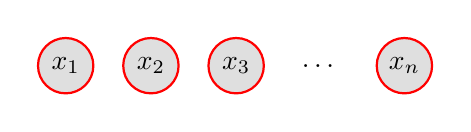
\begin{tikzpicture}
  \node [matrix,matrix anchor=mid, column sep=10pt, row sep=10pt,ampersand replacement=\&] {
    \node (x1) [obs] {$x_1$}; \&
    \node (x2) [obs] {$x_2$}; \&
    \node (x3) [obs] {$x_3$}; \&
    \node (xi) [] {\dots}; \&
    \node (xn) [obs] {$x_n$}; \\
  };
\end{tikzpicture}
\end{block}

\begin{block}{Independent Model}
\centering
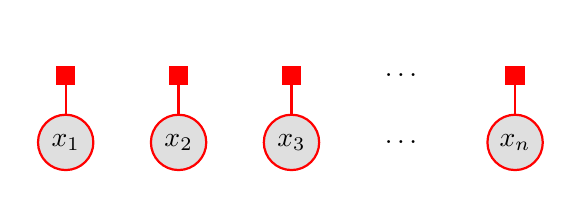
\begin{tikzpicture}
  \node [matrix,matrix anchor=mid, column sep=20pt, row sep=10pt,ampersand replacement=\&] {
    \& \& \& \& \\
    \node (f1) [factor] {}; \&
    \node (f2) [factor] {}; \&
    \node (f3) [factor] {}; \&
    \node (fi) [] {\dots}; \&
    \node (fn) [factor] {}; \\
    \node (x1) [obs] {$x_1$}; \&
    \node (x2) [obs] {$x_2$}; \&
    \node (x3) [obs] {$x_3$}; \&
    \node (xi) [] {\dots}; \&
    \node (xn) [obs] {$x_n$}; \\
  };
  \draw [-] (f1) -- (x1);
  \draw [-] (f2) -- (x2);
  \draw [-] (f3) -- (x3);
  \draw [-] (fi);
  \draw [-] (fn) -- (xn);
\end{tikzpicture}

Factors were trained using samples drawn from the synthetic distribution where the label
for the generating class was hidden.
\end{block}
\end{frame}

\begin{frame}{Results}
  \begin{figure}
    \includegraphics[width=0.7\textwidth]{results/synthetic-all.pdf}
  \end{figure}
\end{frame}


%%%%%%%%%%%%%%%%%%%%%%%%%%%%%%%%%%%%%%%%%%%%%%%%%%%%%%%%%%%%%%%%%%%%%%%%%%%
\section{Conclusion}

\subsection{Summary}
\begin{frame}{Summary}
\begin{itemize}
\item Studies a semantic mapping process
\item Studies novelty detection
\item Proposes a method to perform detection of novel categories
      of a variable when the graph structure is dynamic.
\end{itemize}
\end{frame}

\subsection{Limitations}
\begin{frame}{Limitations}
\begin{block}{Assumption on constant $P(novel)$}
Graph structure plays a role on the likelihood a sample with a novel
category is drawn. Assuming it to be constant is a very strong assumption
that is not expected to hold in all scenarios.
\end{block}
%\begin{block}{Uncertain Sensing}
%The presented methods require calculation of normalized probabilities turning it impossible
%to handle implicit factors.
%\end{block}
\end{frame}

\subsection{Future Work}
\begin{frame}{Future Work}
  \begin{block}{Generalize the Framework}
  Handle novelty on any and more than one variable of the graph and fusing
  all novelty information in a single method in a probabilistic fashion (e.g.\ MAP operation).
  \end{block}
  \begin{block}{Exploit Generative Models}
  Develop methods to be able to explain what the system considers to be known or novel.
  Such that the reason causing novelty can be interpreted.
  \end{block}
\end{frame}
\begin{frame}{Future Work}
  \begin{block}{Learning Graph Structures}
  Graph structure should be considered probabilistic. Methods to handle and probabilistic
  represent knowledge on how the agent detect structures must be develop.
  \end{block}
  \begin{block}{After Detection of Knowledge Gaps}
  What can be done with the detection of novel situations? Can the system be adapted
  to learn and group novel situations? How to perform self-extension?
  \end{block}
\end{frame}

\subsection{Extra Information}
\begin{frame}{Extra}
\begin{block}{Reproducible Research}
All reports and results reproducible from online repository:
\url{https://github.com/andresusanopinto/novelty-detection-thesis}
\end{block}

\begin{block}{Article on EPIA 2011}
\textit{Novelty Detection Using Graphical Models for Semantic Room Classification}
\end{block}
\end{frame}

\appendix
\begin{frame}[allowframebreaks]{Bibliography}
\bibliographystyle{alpha}
\bibliography{refs}
\end{frame}

\begin{frame}
 \titlepage
\end{frame}

\end{document}

